% ============================================================================
%  Chapter 5 -- Results
%  Primary benchmark: CIFAR-100 5x20, seed 42.
% ============================================================================

\chapter{Results}
\label{ch:results}

Every accuracy, restricted-accuracy, backward-transfer, and forgetting value
in this chapter is read directly from the saved result artifacts of the
underlying experiments and independently cross-checked for consistency.
This chapter does not re-derive SimpleAvg, RankExt, knowledge distillation, FactorOrth, or the
open/restricted evaluation protocol, all of which are defined in
Chapter~\ref{ch:methodology}; nor does it restate the dataset, protocol, or
training configuration fixed in Chapter~\ref{ch:experimental-setup}.
Interpretation of \emph{why} the results below occur -- mechanism, cause,
generalisation -- is deferred to Chapter~\ref{ch:discussion-conclusion}.

\section{Evaluation Protocol and Metrics}
\label{sec:ch5-protocol}

The primary results of this chapter are obtained on \textbf{CIFAR-100}
under a \textbf{5-task, 20-class-per-task} class-incremental protocol
($5\times20$), evaluated at \textbf{seed 42}; a supporting second-dataset
evaluation on CUB-200-2011 ($5\times40$, seed 42) is reported in
Section~\ref{sec:ch5-cub}. The metric definitions below apply to both. The
backbone, LoRA configuration, method definitions, and
training procedure are fixed in Chapter~\ref{ch:experimental-setup} and are
not restated here; this section recaps only the metric definitions needed to
read the tables and figures that follow.

\textbf{All-seen (open) accuracy} is the primary continual-learning metric
throughout this chapter: accuracy on a task's own test images, evaluated
against the full, task-agnostic output space of every class introduced up to
and including the current task. Unless stated otherwise, ``accuracy'' in
this chapter means all-seen accuracy.

\textbf{Restricted (task-oracle) accuracy} evaluates the same predictions
against only the current task's own class subset (20 classes on
CIFAR-100, 40 on CUB-200-2011) --- a diagnostic upper
bound on within-task discrimination, not a replacement headline metric.
Restricted accuracy is never described in this chapter as a method's
``true'' or ``actual'' accuracy; it isolates one specific factor
(within-task discriminability) from the task-competition effects that
all-seen accuracy also reflects, and the two are reported side by side
precisely because they can diverge substantially (Section~\ref{sec:ch5-stability}).

\textbf{Classifier rescaling.} After training is complete, the classifier
weight rows associated with each task are rescaled by a positive
task-specific factor to reduce scale imbalance across tasks
(Section~\ref{sec:ch3-calibration}). The backbone, LoRA parameters, and
classifier biases remain unchanged. The same rescaled classifier is then
used for both open and restricted evaluation, and the same classifier
rescaling is applied to all eight methods. Because the biases are
unchanged, restricted accuracy is not mathematically guaranteed to be
invariant to this rescaling.

\textbf{First-task final accuracy} and \textbf{later-tasks mean accuracy}
report, respectively, the open accuracy on task 1 and the mean open accuracy
on tasks 2--5, both measured after the full five-task sequence has
completed. Together they indicate whether a method's aggregate accuracy is
limited by early-task retention, later-task acquisition, or both.

\textbf{Backward transfer (BWT)} follows the standard definition
\parencite{lopezpaz2017gradient}: the mean, over tasks 1 through 4, of the
difference between a task's accuracy at the end of the full sequence and its
accuracy immediately after it was first learned. In the reported values,
the end-of-sequence term is the task's open accuracy in the final model
\emph{after} classifier rescaling, while the ``immediately after learning''
term is evaluated during training, at the end of that task's own training
(from its best-validation checkpoint), \emph{before} any classifier
rescaling. A structural caveat applies
specifically to this thesis's two method families and is stated once, here,
rather than repeated at every table: \textbf{RankExt is a single, persistent
model}, trained sequentially, so its BWT has the standard interpretation --
a genuine measurement of how later training affects earlier-learned tasks in
the same evolving model. \textbf{SimpleAvg is not a single evolving model};
each task is trained as an independent specialist and the five specialists
are combined only once, at the end, by an arithmetic merge
(Chapter~\ref{ch:methodology}). SimpleAvg's reported BWT therefore uses each
specialist's own accuracy, immediately after its independent training, as
the ``immediately after learning'' reference point --- a pre-merge
specialist diagonal substitute, not a measurement of sequential interference
in an evolving model. The two families' BWT values are reported in the same
column for compactness but are \textbf{not structurally equivalent} and
should not be read as directly comparable to one another.

\textbf{Forgetting} \parencite{chaudhry2018riemannian} is reported only for
RankExt, where it is well-defined (the mean, over tasks 1--4, of each task's
best-ever observed accuracy minus its accuracy at the end of the sequence).
Unlike BWT, forgetting is computed entirely from the in-training
evaluations made after each task, before classifier rescaling --- the same
values that form the $R_{i,j}$ matrices of Section~\ref{sec:ch5-rankext}.
It is structurally undefined for SimpleAvg, which has no sequential model to
forget from, and is reported as ``---'' for every SimpleAvg row --- never as
0, which would imply a measured absence of forgetting rather than a metric
that does not apply.



All results reported as primary in this chapter come from a \textbf{single
production run at a single seed (42)}. No statistical significance test was
performed anywhere in this chapter. Differences are described as ``observed
in this run'' or ``at this seed,'' never as ``statistically significant,''
``robust,'' or ``consistent'' across replications; this limitation is
restated concisely in Section~\ref{sec:ch5-summary} rather than after every
individual number.

\section{CIFAR-100 Main Results}
\label{sec:ch5-main-results}

The canonical Chapter-5 benchmark compares \textbf{eight} methods under the
CIFAR-100 $5\times20$ protocol at seed 42. All KD-bearing configurations use
a distillation temperature of $T=2$, as specified in
Chapter~\ref{ch:experimental-setup}. No result from any other experiment is
merged into this benchmark; the CUB-200-2011 evaluation is reported
separately in Section~\ref{sec:ch5-cub}, and the refinement and
protocol-diagnostic experiments in Section~\ref{sec:ch5-ablation}.

Table~\ref{tab:ch5-main-compact} reports all-seen and restricted accuracy
for the eight canonical methods.

\begin{table}[htbp]
\centering
\begin{tabularx}{\textwidth}{@{}X r r@{}}
\toprule
\textbf{Method} & \textbf{All-seen (\%)} & \textbf{Restricted (\%)} \\
\midrule
SimpleAvg & 75.16 & 92.28 \\
SimpleAvg + KD & 75.21 & 92.86 \\
SimpleAvg + FactorOrth & 74.02 & 91.97 \\
SimpleAvg + FactorOrth + KD & 73.22 & 92.96 \\
RankExt & 34.99 & 91.03 \\
RankExt + KD + Protect & 65.01 & 94.10 \\
RankExt + FactorOrth & 41.00 & 93.03 \\
RankExt + FactorOrth + KD + Protect & 70.76 & 94.78 \\
\bottomrule
\end{tabularx}
\caption[Main CIFAR-100 8-method benchmark]{All-seen and restricted accuracy
for the eight canonical methods, CIFAR-100 $5\times20$, the primary benchmark, seed 42.}
\label{tab:ch5-main-compact}
\end{table}

\begin{figure}[htbp]
\centering
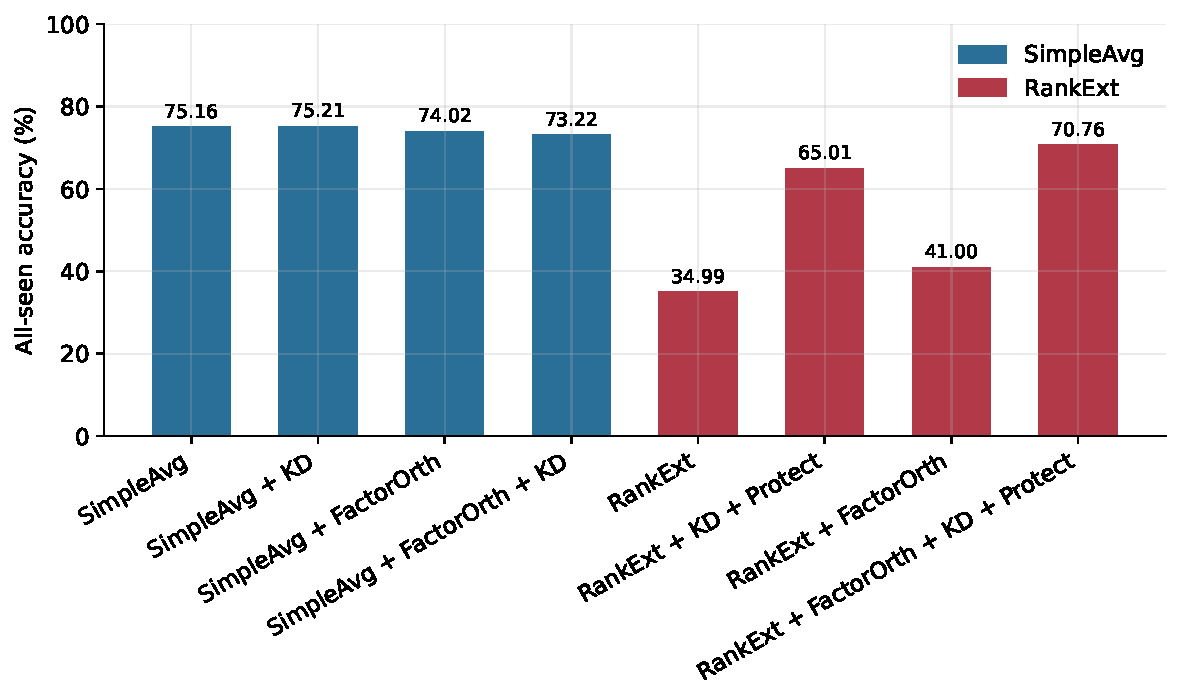
\includegraphics[width=0.95\textwidth]{figures/chapter5/cifar100_allseen_accuracy.pdf}
\caption[All-seen accuracy, main benchmark]{All-seen accuracy for the eight
canonical methods, coloured by family, zero-based axis. Source:
\texttt{chapter5\_cifar100\_8method\_main.csv}.}
\label{fig:ch5-allseen}
\end{figure}

The extended version of Table~\ref{tab:ch5-main-compact}, additionally
reporting first-task accuracy, later-tasks-mean accuracy, BWT, and
forgetting for all eight methods, is given as
Table~\ref{tab:ch5-main-extended} in Section~\ref{sec:ch5-summary}.

Two patterns are immediately visible and structure the remainder of this
chapter. The four SimpleAvg variants occupy a narrow band, from 73.22\% to
75.21\% --- a 1.99-percentage-point range. The four RankExt variants span a
much wider range, from 34.99\% to 70.76\% --- a 35.77-percentage-point
range, roughly eighteen times larger than SimpleAvg's own spread. The
highest observed SimpleAvg result in this run (SimpleAvg + KD, 75.21\%) and
the highest observed RankExt result in this run (RankExt + FactorOrth + KD +
Protect, 70.76\%) differ by \textbf{4.45 percentage points}, with SimpleAvg
ahead (Figure~\ref{fig:ch5-best-per-family}).
This single-seed gap is the cleanest one-number summary of this benchmark,
but should not be read as a significance test.

\begin{figure}[htbp]
\centering
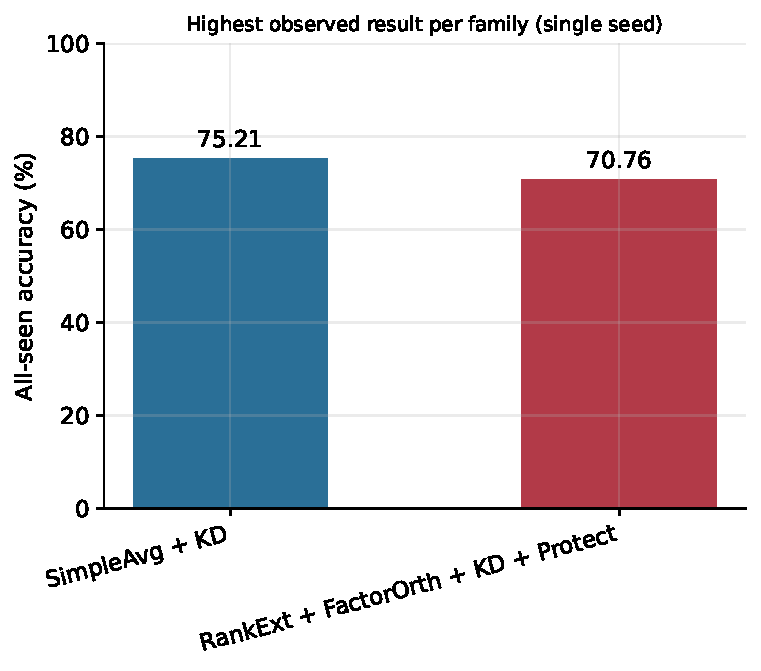
\includegraphics[width=0.55\textwidth]{figures/chapter5/cifar100_best_per_family.pdf}
\caption[Best result per family]{Best observed all-seen accuracy per family:
SimpleAvg + KD (75.21\%) versus RankExt + FactorOrth + KD + Protect
(70.76\%). A single-seed headline comparison, not a statistical significance
test.}
\label{fig:ch5-best-per-family}
\end{figure}

Read narratively: SimpleAvg establishes a strong baseline near 75\% without
requiring any auxiliary objective, and its three auxiliary-loss variants do
not move materially away from that baseline in either direction. RankExt's
plain configuration is far weaker, and the configurations with auxiliary
objectives reach substantially higher all-seen accuracy, up to 70.76\%. Sections~\ref{sec:ch5-simpleavg} and~\ref{sec:ch5-rankext}
examine each family in turn; the \emph{reasons} for this asymmetry are
deferred to Chapter~\ref{ch:discussion-conclusion}.

\section{CUB-200-2011 Cross-Dataset Evaluation}
\label{sec:ch5-cub}

The CUB-200-2011 experiment evaluates the same eight methods on a second
dataset, under the $5\times40$ protocol with seed 42
(Section~\ref{sec:ch4-datasets}). It is a supporting cross-dataset
evaluation, not a second primary benchmark: in addition to the dataset
itself, the class count, classes per step, classifier size, and
preprocessing differ from CIFAR-100, and the refined CUB-200-2011
configuration uses a RankExt classifier-head learning-rate multiplier of
$\times2$ instead of the canonical $\times1$
(Table~\ref{tab:ch4-cub-config}). Table~\ref{tab:ch5-cub-main} reports the
results.

\begin{table}[htbp]
\centering
\begin{tabularx}{\textwidth}{@{}X r r r r@{}}
\toprule
\textbf{Method} & \textbf{All-seen (\%)} & \textbf{Restricted (\%)} & \textbf{BWT} & \textbf{Forgetting} \\
\midrule
SimpleAvg & 69.47 & 91.25 & $-$0.241 & --- \\
SimpleAvg + KD & 68.69 & 91.94 & $-$0.266 & --- \\
SimpleAvg + FactorOrth & 68.33 & 91.05 & $-$0.259 & --- \\
SimpleAvg + FactorOrth + KD & 67.24 & 91.74 & $-$0.288 & --- \\
RankExt & 20.26 & 78.12 & $-$0.891 & 0.890 \\
RankExt + KD + Protect & 45.27 & 87.78 & $-$0.547 & 0.589 \\
RankExt + FactorOrth & 20.82 & 79.58 & $-$0.885 & 0.884 \\
RankExt + FactorOrth + KD + Protect & 63.43 & 88.39 & $-$0.532 & 0.570 \\
\bottomrule
\end{tabularx}
\caption[CUB-200-2011 8-method results]{CUB-200-2011 $5\times40$, seed 42:
all-seen and restricted accuracy, BWT, and forgetting for the eight methods.
BWT and forgetting follow the definitions and evaluation stages of
Section~\ref{sec:ch5-protocol}; forgetting is reported for RankExt only.
As on CIFAR-100, FactorOrth is applied to the reconstructed dense updates
for SimpleAvg ($\lambda=20$) and in the low-rank factor space for RankExt
($\lambda=50$).}
\label{tab:ch5-cub-main}
\end{table}

\textbf{SimpleAvg.} In this single-seed CUB experiment, none of the
auxiliary SimpleAvg configurations improves on the plain 69.47\% baseline:
relative to plain SimpleAvg, KD changes all-seen accuracy by $-$0.78
percentage points, FactorOrth by $-$1.14 points, and their combination by
$-$2.23 points. Restricted accuracy stays between 91.05\% and 91.94\% for
all four variants.

\textbf{RankExt.} Plain RankExt reaches 20.26\%. FactorOrth alone has only a
small observed effect ($+$0.55 percentage points, to 20.82\%). The
KD+Protect configuration, which combines knowledge distillation with the
projected feature-protection term, raises all-seen accuracy by 25.01 points
to 45.27\%, and the combined FactorOrth + KD + Protect configuration
produces the highest observed RankExt result on CUB-200-2011, 63.43\%
($+$43.17 points over plain and $+$18.16 points over KD+Protect). As on
CIFAR-100, the contributions of knowledge distillation and the projected
feature-protection term are not isolated. The highest observed SimpleAvg
result (69.47\%) and the highest observed RankExt result (63.43\%) show a
6.04-percentage-point difference in this single-seed CUB experiment.
Restricted accuracy for RankExt ranges from 78.12\% to 88.39\%, which is
lower than both the CUB-200-2011 SimpleAvg values and the CIFAR-100 RankExt
values (91.03\%--94.78\%).

\begin{table}[htbp]
\centering
\begin{tabularx}{\textwidth}{@{}X r r@{}}
\toprule
\textbf{Method} & \shortstack[r]{\textbf{CIFAR-100 $5\times20$}\\\textbf{all-seen (\%)}} & \shortstack[r]{\textbf{CUB-200-2011 $5\times40$}\\\textbf{all-seen (\%)}} \\
\midrule
SimpleAvg & 75.16 & 69.47 \\
SimpleAvg + KD & 75.21 & 68.69 \\
SimpleAvg + FactorOrth & 74.02 & 68.33 \\
SimpleAvg + FactorOrth + KD & 73.22 & 67.24 \\
RankExt & 34.99 & 20.26 \\
RankExt + KD + Protect & 65.01 & 45.27 \\
RankExt + FactorOrth & 41.00 & 20.82 \\
RankExt + FactorOrth + KD + Protect & 70.76 & 63.43 \\
\bottomrule
\end{tabularx}
\caption[CIFAR-100 versus CUB-200-2011 all-seen accuracy]{All-seen accuracy
on the CIFAR-100 primary benchmark and the CUB-200-2011 evaluation (single
seed each). This is a descriptive comparison, not a controlled estimate of
the dataset effect: the two runs also differ in class count, classes per
step, classifier size, preprocessing, and the RankExt classifier-head
learning-rate multiplier ($\times1$ on CIFAR-100, $\times2$ on
CUB-200-2011).}
\label{tab:ch5-cub-vs-cifar}
\end{table}

\textbf{Relation to CIFAR-100.} Table~\ref{tab:ch5-cub-vs-cifar} places the
two datasets side by side. The CUB experiment reproduces the main
qualitative family-level pattern observed on CIFAR-100, although the runs
are not a strict dataset-only controlled comparison because the refined CUB
configuration uses a $\times2$ RankExt classifier-head multiplier. On both
datasets, SimpleAvg is strong without auxiliary objectives and none of its
auxiliary variants clearly improves on the plain baseline; plain RankExt is
substantially weaker; FactorOrth alone does not resolve that weakness; the
KD+Protect-bearing configurations show much larger recovery; and the
combined configuration is the highest observed RankExt result without
reaching the highest observed SimpleAvg result. All-seen accuracy is
lower on CUB-200-2011 for every method, and the differences between the two
datasets are not attributed to dataset properties alone.

\section{SimpleAvg Analysis}
\label{sec:ch5-simpleavg}

Sections~\ref{sec:ch5-simpleavg}--\ref{sec:ch5-ablation} return to the
CIFAR-100 primary benchmark.

This section examines whether any of the three auxiliary mechanisms
available to SimpleAvg --- knowledge distillation (KD), FactorOrth, or their
combination --- improves on the plain arithmetic-merge baseline. For
SimpleAvg, FactorOrth is applied to the reconstructed dense updates
($\lambda=20$), whereas for RankExt it is applied directly in the low-rank
factor space ($\lambda=50$) (Section~\ref{sec:ch3-factororth}).

Table~\ref{tab:ch5-simpleavg} reports each SimpleAvg variant's delta from
plain SimpleAvg (75.16\%), alongside first-task and later-tasks-mean
accuracy.

\begin{table}[htbp]
\centering
\begin{tabularx}{\textwidth}{@{}>{\raggedright\arraybackslash}X r r r r r@{}}
\toprule
\textbf{Method} & \shortstack[r]{\textbf{All-seen}\\\textbf{(\%)}} & \shortstack[r]{\textbf{$\Delta$ vs.\ plain}\\\textbf{(pp)}} & \shortstack[r]{\textbf{First-task}\\\textbf{(\%)}} & \shortstack[r]{\textbf{Later-tasks}\\\textbf{mean (\%)}} & \shortstack[r]{\textbf{Restricted}\\\textbf{(\%)}} \\
\midrule
SimpleAvg (plain) & 75.16 & --- & 77.75 & 74.51 & 92.28 \\
SimpleAvg + KD & 75.21 & +0.05 & 68.25 & 76.95 & 92.86 \\
SimpleAvg + FactorOrth & 74.02 & $-$1.14 & 76.60 & 73.38 & 91.97 \\
SimpleAvg + FactorOrth + KD & 73.22 & $-$1.94 & 57.55 & 77.14 & 92.96 \\
\bottomrule
\end{tabularx}
\caption[SimpleAvg family results]{SimpleAvg family: all-seen accuracy,
delta from plain, first-task, later-tasks mean, and restricted accuracy.}
\label{tab:ch5-simpleavg}
\end{table}

\begin{figure}[htbp]
\centering
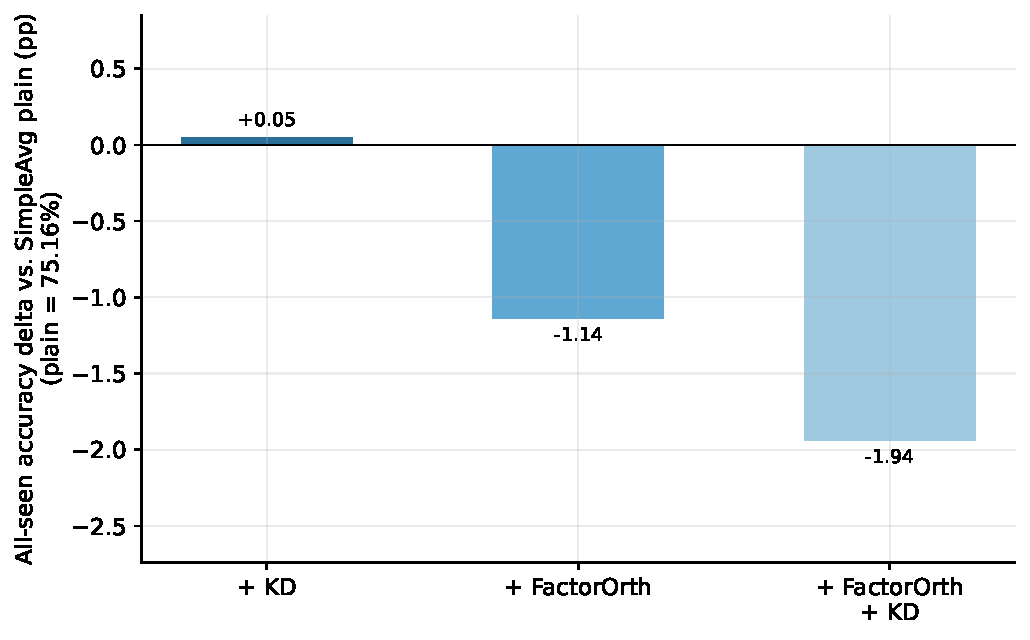
\includegraphics[width=0.75\textwidth]{figures/chapter5/cifar100_simpleavg_delta_from_plain.pdf}
\caption[SimpleAvg delta from plain]{All-seen accuracy delta of each
SimpleAvg variant relative to plain SimpleAvg, with a zero reference line.}
\label{fig:ch5-sa-delta}
\end{figure}

The +0.05 percentage-point difference between SimpleAvg + KD and plain
SimpleAvg is too small to support a meaningful improvement claim from this
single-seed experiment. Both FactorOrth
variants score below plain SimpleAvg: FactorOrth alone by 1.14 percentage
points, FactorOrth combined with KD by 1.94 percentage points, the largest
deviation from plain among the four SimpleAvg variants. None of the three
auxiliary configurations produces a clear all-seen improvement over the
plain baseline.

The near-tied all-seen numbers mask a larger redistribution across tasks.
SimpleAvg + KD's first-task accuracy (68.25\%) is 9.50 percentage points
below plain SimpleAvg's (77.75\%), while its later-tasks mean (76.95\%) is
2.44 points above plain's (74.51\%); restricted accuracy is also higher for
the KD variant (92.86\% vs.\ 92.28\%). SimpleAvg + FactorOrth + KD shows the
same direction at a larger magnitude --- first-task accuracy 57.55\% (20.20
points below plain), later-tasks mean 77.14\% (the highest later-tasks value
among the four SimpleAvg variants), restricted accuracy 92.96\% (also the
highest of the four). SimpleAvg + FactorOrth alone, without KD, does not show
this redistribution: its first-task accuracy (76.60\%) and later-tasks mean
(73.38\%) both stay close to plain's. This chapter reports the
redistribution as a factual pattern --- accuracy moves from the first task
toward later tasks whenever KD is present, roughly in proportion to how it
is combined --- without attributing a cause to it;
Chapter~\ref{ch:discussion-conclusion} addresses why.

\begin{figure}[htbp]
\centering
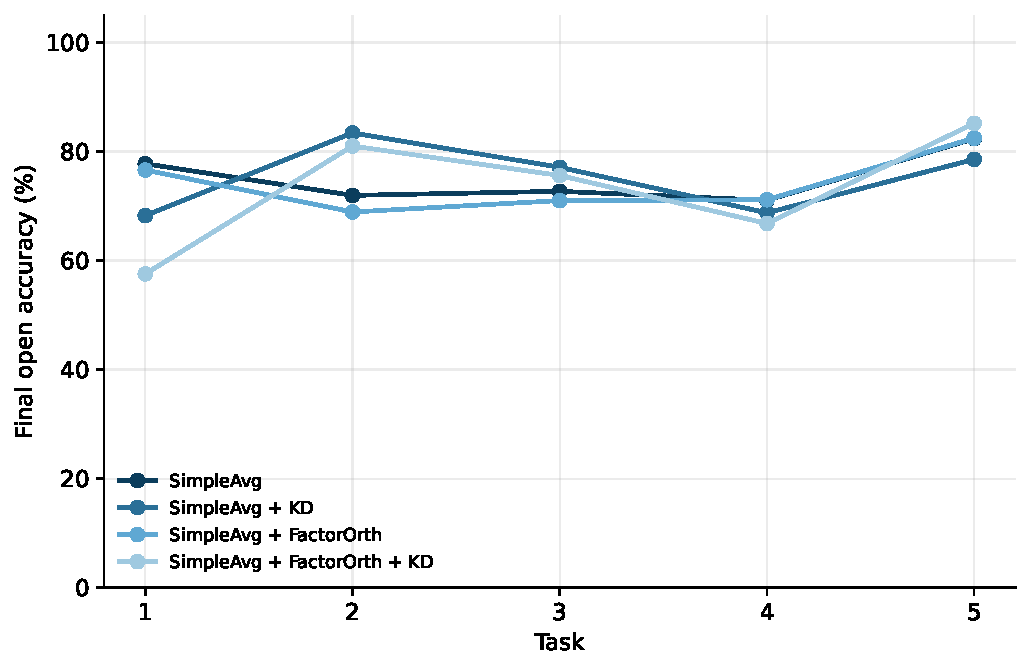
\includegraphics[width=0.75\textwidth]{figures/chapter5/cifar100_sa_per_task_final_open.pdf}
\caption[SimpleAvg per-task final open accuracy]{Final (post-sequence) open
accuracy for each of the five tasks, per SimpleAvg variant.}
\label{fig:ch5-sa-per-task-open}
\end{figure}

\begin{figure}[htbp]
\centering
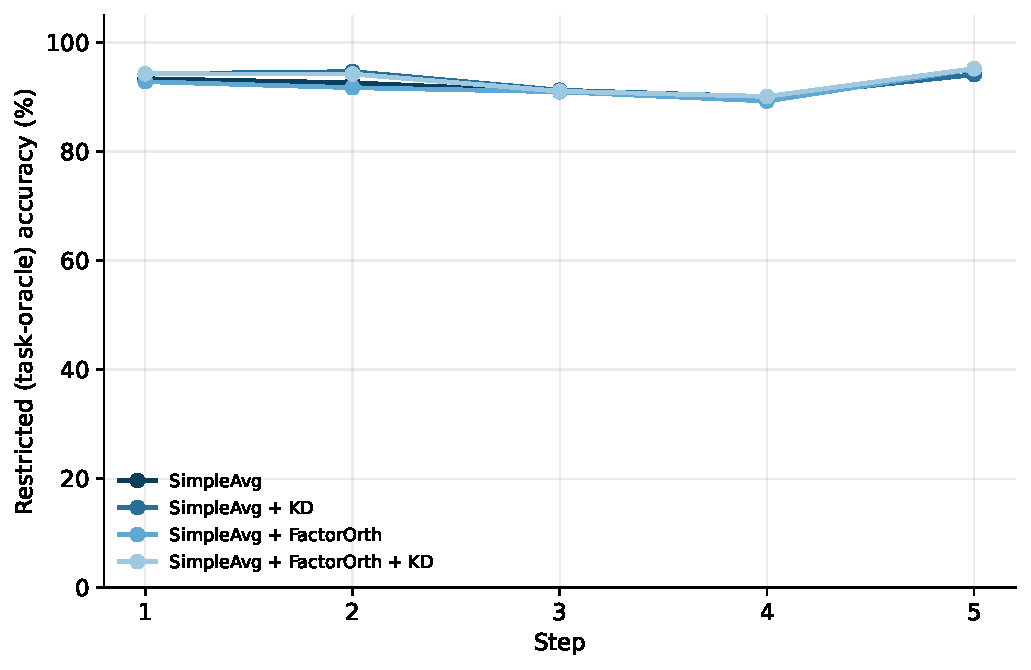
\includegraphics[width=0.75\textwidth]{figures/chapter5/cifar100_sa_per_task_restricted.pdf}
\caption[SimpleAvg per-task restricted accuracy]{Restricted (task-oracle)
accuracy for each of the five tasks, per SimpleAvg variant.}
\label{fig:ch5-sa-per-task-restricted}
\end{figure}

Per-task detail (Figures~\ref{fig:ch5-sa-per-task-open}
and~\ref{fig:ch5-sa-per-task-restricted}) shows this redistribution is not
uniform across the four non-final tasks: for both KD-bearing variants, task
1's open accuracy is the most affected, while tasks 2--4 move by smaller and
less consistent amounts. At the aggregate level, restricted accuracy
across the four SimpleAvg variants spans only 0.99 percentage points, from
91.97\% to 92.96\%. The per-task restricted results
(Figure~\ref{fig:ch5-sa-per-task-restricted}) provide the corresponding
task-level detail.

\section{RankExt Analysis}
\label{sec:ch5-rankext}

This section reports how RankExt's four variants perform relative to plain
RankExt, and presents the per-step, per-task retention trajectory underlying
the aggregate numbers.

Table~\ref{tab:ch5-rankext} reports each RankExt variant's all-seen accuracy
and its recovery over plain RankExt (34.99\%).

\begin{table}[htbp]
\centering
\begin{tabularx}{\textwidth}{@{}X r r r r r@{}}
\toprule
\textbf{Method} & \textbf{All-seen (\%)} & \textbf{$\Delta$ vs.\ plain (pp)} & \textbf{Restricted (\%)} & \textbf{BWT} & \textbf{Forgetting} \\
\midrule
RankExt (plain) & 34.99 & --- & 91.03 & $-$0.7527 & 0.8130 \\
RankExt + FactorOrth & 41.00 & +6.01 & 93.03 & $-$0.6789 & 0.7646 \\
RankExt + KD + Protect & 65.01 & +30.02 & 94.10 & $-$0.2574 & 0.3269 \\
RankExt + FactorOrth + KD + Protect & 70.76 & +35.77 & 94.78 & $-$0.1584 & 0.2474 \\
\bottomrule
\end{tabularx}
\caption[RankExt family results]{RankExt family: all-seen accuracy, delta
from plain, restricted accuracy, BWT, and forgetting.}
\label{tab:ch5-rankext}
\end{table}

\begin{figure}[htbp]
\centering
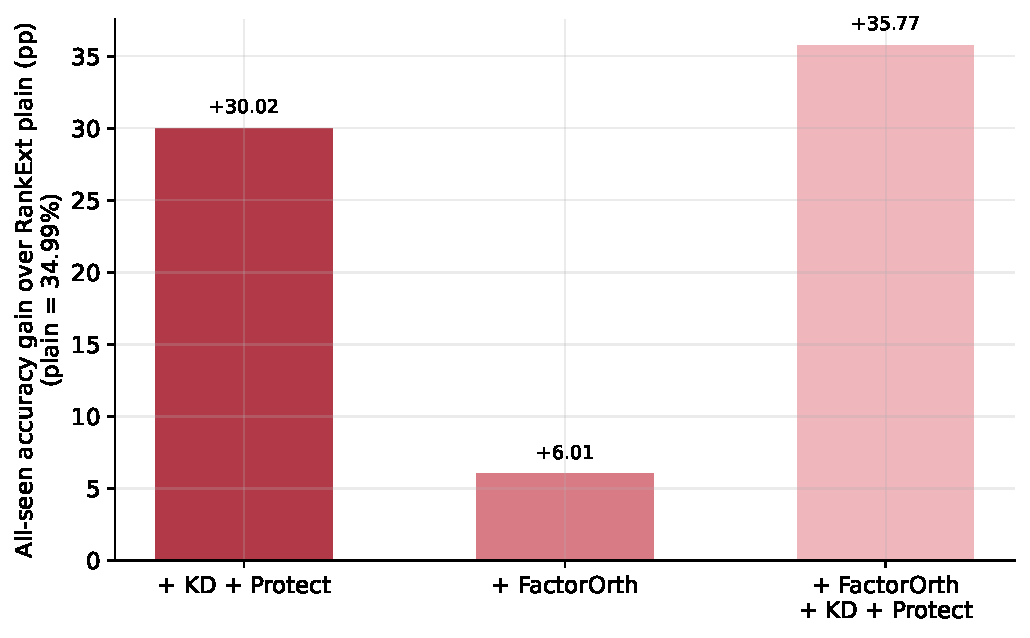
\includegraphics[width=0.75\textwidth]{figures/chapter5/cifar100_rankext_recovery_over_plain.pdf}
\caption[RankExt recovery over plain]{All-seen accuracy gain of each
enhanced RankExt variant over plain RankExt (34.99\%).}
\label{fig:ch5-rankext-recovery}
\end{figure}

Every auxiliary configuration improves on plain RankExt, and the
improvements are far from equal in size. The FactorOrth-only configuration
recovers 6.01 percentage points. The KD+Protect configuration combines
knowledge distillation with the projected feature-protection term; these
two components are not isolated from one another by a separate arm in this
benchmark. It recovers 30.02 percentage points. The combined configuration
(FactorOrth together with KD+Protect) reaches the highest observed RankExt
result in this run, 70.76\%, 35.77 percentage points above plain and 5.75
points above the KD+Protect configuration alone. BWT and forgetting improve
monotonically in the same order, consistent with the all-seen ranking. The
largest observed improvement within RankExt is therefore associated with
the KD+Protect-bearing configurations; because knowledge distillation and
projected feature protection are always active together in this benchmark,
this chapter does not attribute the improvement to either component in
isolation.

\textbf{$R_{i,j}$ trajectories.} For a sequentially-trained, persistent
model such as RankExt, this chapter additionally reports the full retention
matrix $R_{i,j}$: the open (all-seen) accuracy on task $j$, evaluated after
training has completed sequentially through task $i$ ($j \le i$). Each row
$i$ of $R_{i,j}$ is evaluated during training, immediately after task $i$
has been trained (from its best-validation checkpoint), before classifier
rescaling, with predictions taken over the full 100-way classifier output;
at $i=5$ this coincides with evaluation over all seen classes. The final
row of $R_{i,j}$ therefore describes the model before classifier rescaling,
whereas the final accuracies reported in Table~\ref{tab:ch5-main-extended}
describe the same weights after it. The two are not interchangeable: for
plain RankExt, for example, task 1 reaches 6.40\% in the final row of
$R_{i,j}$ and 11.70\% after classifier rescaling.

Figure~\ref{fig:ch5-rij-comparison} shows the four RankExt matrices together
with the SimpleAvg family, on one shared 0--100\% colour scale. Beneath
each RankExt matrix, a separate ``Final'' row gives the per-task open
accuracy of the final model after classifier rescaling. SimpleAvg does not
maintain a persistent merged model at intermediate steps, so it has no
$R_{i,j}$ trajectory; its panels show only the corresponding ``Final'' row
of the merged model, which is directly comparable to the ``Final'' rows of
the RankExt panels.

\begin{figure}[htbp]
\centering
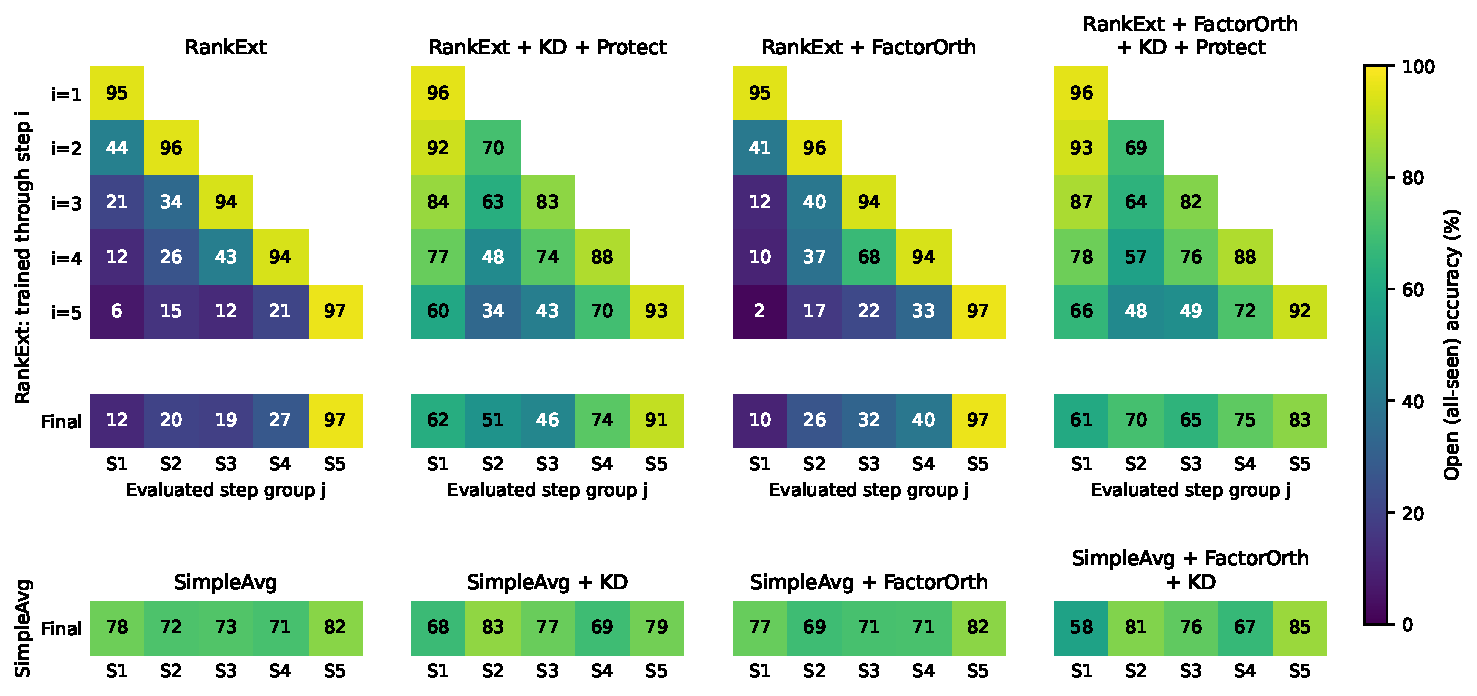
\includegraphics[width=\textwidth]{figures/chapter5/cifar100_retention_rankext_Rij_simpleavg_final.pdf}
\caption[Retention matrices and final per-task accuracy]{Open (all-seen)
accuracy per task group, shared 0--100\% colour scale. Top row: for
RankExt, the panels show the sequential $R_{i,j}$ trajectory (accuracy on
task $j$ after training through task $i$, evaluated before classifier
rescaling), followed by a separate ``Final'' row for the final model after
classifier rescaling. Bottom row: because SimpleAvg does not maintain a
persistent merged model at intermediate steps, the SimpleAvg panels report
only final merged-model per-task accuracies, after classifier rescaling.}
\label{fig:ch5-rij-comparison}
\end{figure}

Plain RankExt's matrix shows every task's own diagonal accuracy above 93\%
at the step it was learned (95.40\%, 95.70\%, 94.05\%, 93.90\%, 97.05\% for
tasks 1--5 respectively), while its off-diagonal, older-task cells decline
steeply as later tasks are trained: task 1's open accuracy, for example,
falls from 95.40\% (its own diagonal) to 43.50\% after task 2 is trained,
20.75\% after task 3, 12.10\% after task 4, and 6.40\% after task 5. The
combined configuration's matrix shows the same qualitative decline in
direction but at a markedly smaller magnitude: task 1's open accuracy after
task 5 is 66.40\%, compared with plain RankExt's 6.40\% at the same matrix
position. The KD+Protect configuration's matrix (task 1 at 60.10\% after
task 5) and the FactorOrth-only configuration's matrix (task 1 at 1.95\%
after task 5, the lowest value observed at that matrix position among the
four configurations) sit, respectively, close to and below the combined
configuration's retention level. These are reported here as factual
trajectory observations; a mechanistic account of what specifically differs
between the four configurations' retention behaviour is given in
Chapter~\ref{ch:discussion-conclusion}.

\section{Stability, Plasticity, and Open-vs-Restricted Performance}
\label{sec:ch5-stability}

This section reports the aggregate open-versus-restricted comparison across
all eight methods.

\begin{figure}[htbp]
\centering
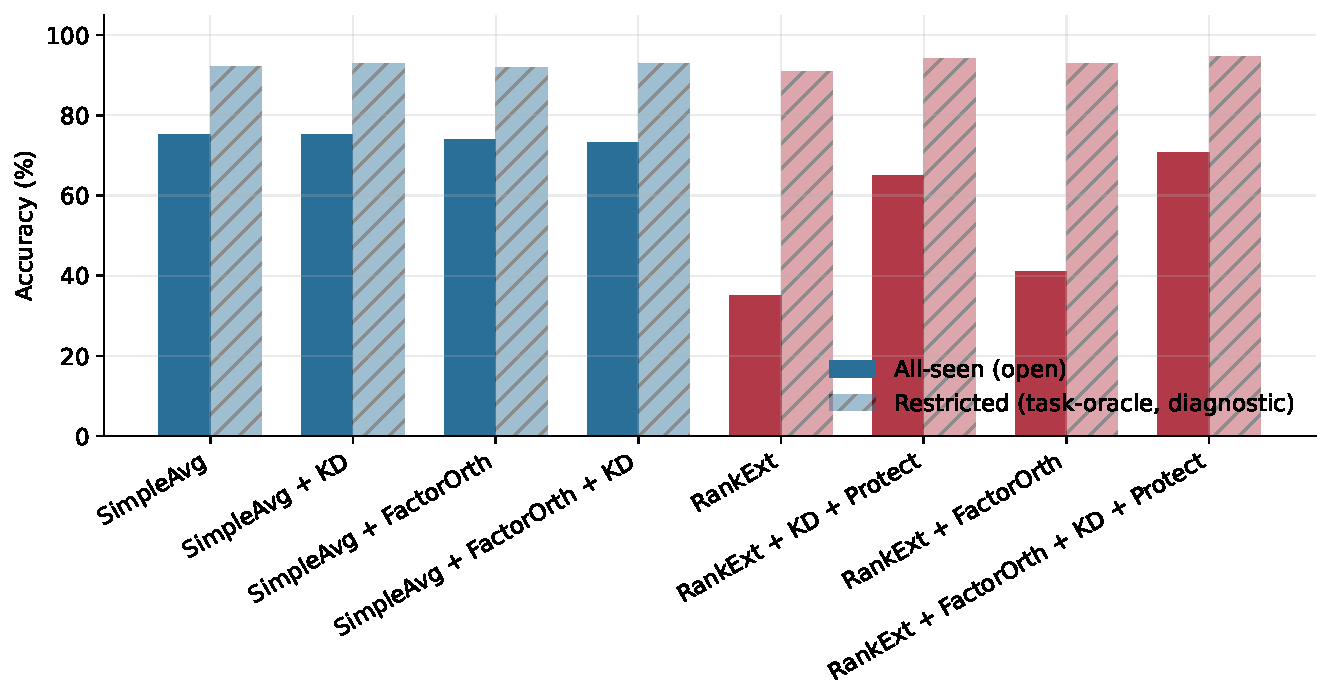
\includegraphics[width=0.85\textwidth]{figures/chapter5/cifar100_open_vs_restricted.pdf}
\caption[Open vs.\ restricted accuracy]{All-seen (open) vs.\ restricted
(task-oracle, diagnostic) accuracy for all eight methods.}
\label{fig:ch5-open-vs-restricted}
\end{figure}

Across all eight methods, restricted (task-oracle) accuracy falls in a
\textbf{91.03\%--94.78\%} range (Figure~\ref{fig:ch5-open-vs-restricted}) ---
a 3.75-percentage-point spread, far narrower than the 35.77-point spread
observed in all-seen accuracy among the four RankExt variants alone
(Section~\ref{sec:ch5-rankext}).

\begin{figure}[htbp]
\centering
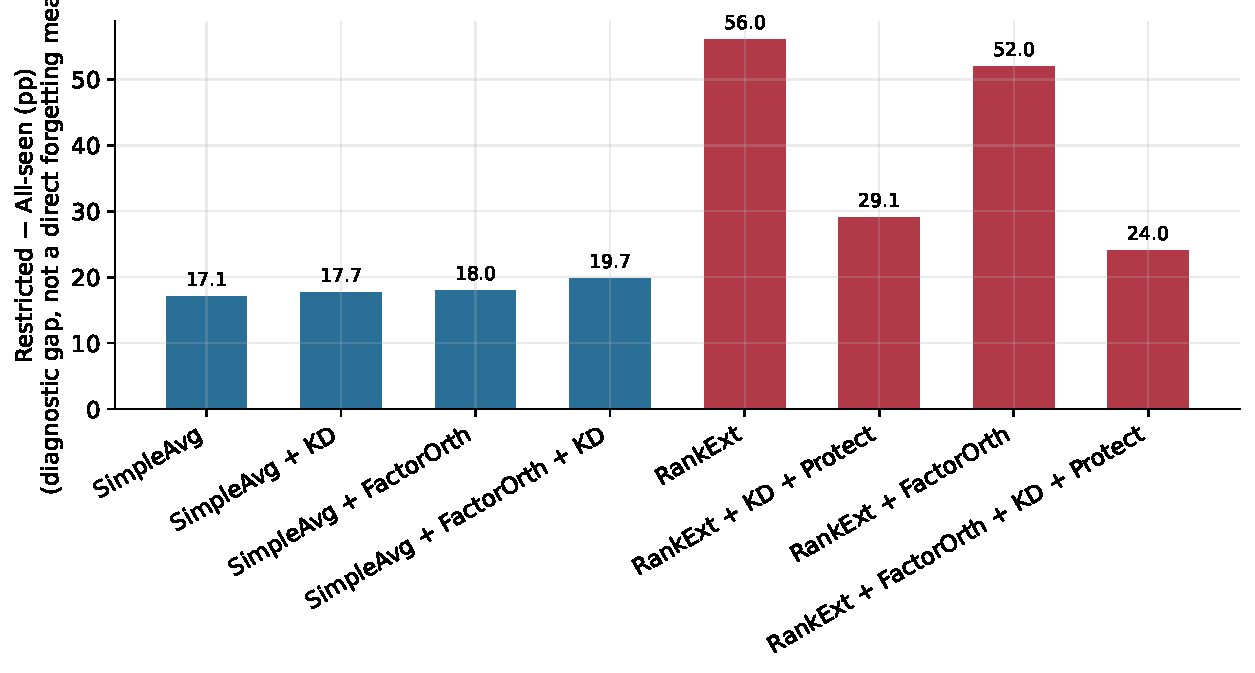
\includegraphics[width=0.85\textwidth]{figures/chapter5/cifar100_open_restricted_gap.pdf}
\caption[Open--restricted gap]{Restricted-minus-open accuracy gap per
method --- a diagnostic indicator of cross-task competition, not a direct
measure of catastrophic forgetting.}
\label{fig:ch5-open-restricted-gap}
\end{figure}

The open/restricted gap (restricted minus all-seen,
Figure~\ref{fig:ch5-open-restricted-gap}) is comparatively small and
narrow-ranging for every SimpleAvg variant (17.12 to 19.74 percentage
points, widening somewhat for the KD-bearing variants because of the
first-task redistribution described in Section~\ref{sec:ch5-simpleavg}) and
substantially larger for the two RankExt variants without KD+Protect:
plain RankExt's restricted accuracy (91.03\%) exceeds its
all-seen accuracy (34.99\%) by \textbf{56.04 percentage points}, the largest
gap of any method in this benchmark. RankExt + FactorOrth shows a comparably
large gap (93.03\% $-$ 41.00\% = 52.03 points). The two configurations that
include KD+Protect show substantially smaller gaps: RankExt + KD + Protect
(94.10\% $-$ 65.01\% = 29.09 points) and the combined configuration (94.78\%
$-$ 70.76\% = 24.02 points).

The gap indicates that within-task discrimination is substantially stronger
than task-agnostic discrimination across all seen classes, for every
RankExt configuration measured in this benchmark, and most severely for the
two configurations without KD+Protect. This is reported here as an observed
pattern. Restricted evaluation removes cross-task class competitors from the
decision rule and therefore provides a diagnostic view of within-task
discrimination; it does not identify the cause of the open-accuracy
shortfall, possible readings of which are examined in
Chapter~\ref{ch:discussion-conclusion}.

\begin{figure}[htbp]
\centering
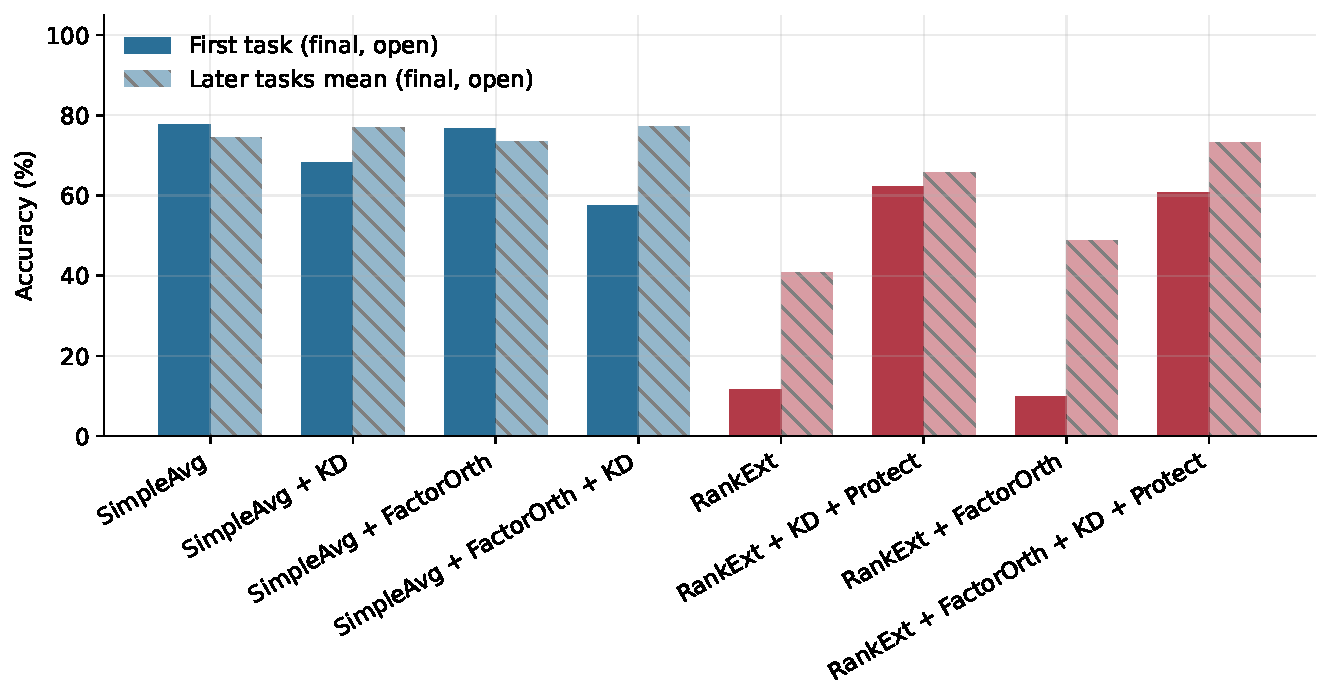
\includegraphics[width=0.85\textwidth]{figures/chapter5/cifar100_first_vs_later_tasks.pdf}
\caption[First-task vs.\ later-tasks accuracy]{First-task and later-tasks
mean accuracy for all eight methods.}
\label{fig:ch5-first-vs-later}
\end{figure}

Figure~\ref{fig:ch5-first-vs-later} presents first-task and later-tasks-mean
accuracy for all eight methods together, consolidating the per-family
patterns already reported in Sections~\ref{sec:ch5-simpleavg}
and~\ref{sec:ch5-rankext}: SimpleAvg's KD-bearing variants trade first-task
accuracy for later-tasks accuracy at roughly constant all-seen accuracy.
Within RankExt, the KD+Protect-bearing configurations substantially increase
both first-task and later-tasks accuracy relative to plain RankExt, whereas
FactorOrth alone increases later-tasks accuracy (48.79\% vs.\ 40.81\%) but
not first-task accuracy (9.85\% vs.\ 11.70\%)
(Table~\ref{tab:ch5-main-extended}).

\section{Parameter and Rank Efficiency}
\label{sec:ch5-efficiency}

This thesis is specifically concerned with LoRA-based merging and rank
extension; this section reports the structural parameter cost of each
family alongside the accuracy results of Sections~\ref{sec:ch5-main-results},
\ref{sec:ch5-simpleavg}, and~\ref{sec:ch5-rankext}, so that Chapter 5's
headline comparison is not accuracy-only.

Both families target the same 24 LoRA modules (\texttt{q\_proj} and
\texttt{v\_proj} in each of the 12 CLIP ViT-B/16 vision-encoder layers,
hidden size 768). SimpleAvg trains a fixed rank-80 adapter independently for
each of the five tasks; RankExt trains a cumulative adapter that grows by a
fixed rank-16 increment at each task, reaching a cumulative rank of 80 only
at the fifth and final task (Figure~\ref{fig:ch5-rank-growth}). The two rank
trajectories reach the same final value by construction, but represent
structurally different histories: SimpleAvg's rank-80 at every task is a
\emph{new, independent} specialist, not an accumulation; RankExt's rank-80
at task 5 is the sum of five smaller, sequentially-added, never-retrained
blocks. At the final training step, the SimpleAvg specialist rank and the
RankExt cumulative active rank are both 80; this does not imply that
SimpleAvg's final averaged dense update is itself rank-80 constrained.

\begin{figure}[htbp]
\centering
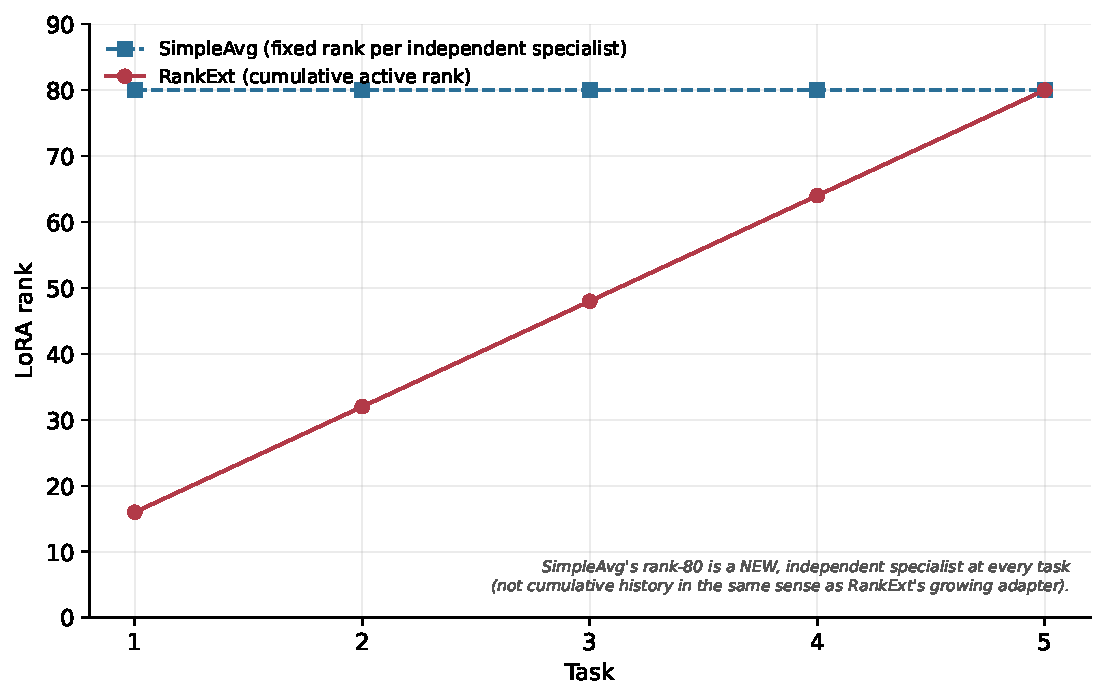
\includegraphics[width=0.8\textwidth]{figures/chapter5/cifar100_rank_growth.pdf}
\caption[LoRA rank growth]{LoRA rank used by each family across the 5-task
sequence. SimpleAvg's rank-80 is a new, independent specialist at every
task, not cumulative history in the same sense as RankExt's growing
adapter.}
\label{fig:ch5-rank-growth}
\end{figure}

Table~\ref{tab:ch5-param-efficiency} summarises the comparison.

\begin{table}[htbp]
\centering
\begin{tabularx}{\textwidth}{@{}X X X@{}}
\toprule
\textbf{Property} & \textbf{SimpleAvg} & \textbf{RankExt} \\
\midrule
Rank behaviour & Fixed rank 80, fresh independent specialist per task & Growing cumulative rank: $16{\to}32{\to}48{\to}64{\to}80$ \\
New trainable LoRA params, per task & 2{,}949{,}120 (constant) & 589{,}824 (constant) \\
LoRA parameter volume touched across all 5 tasks & 14{,}745{,}600 (5 independent adapters) & 2{,}949{,}120 (5 blocks, each trained once) \\
Final deployed LoRA overhead & 0 if the averaged delta is fused into the base model, or 14{,}155{,}776 if the dense delta is instead stored separately & 2{,}949{,}120 (kept in low-rank, additive form) \\
Final deployed classifier & 76{,}900 & 76{,}900 \\
\bottomrule
\end{tabularx}
\caption[Parameter/rank-efficiency comparison]{Structural parameter/rank
efficiency comparison, SimpleAvg vs.\ RankExt, the primary benchmark.}
\label{tab:ch5-param-efficiency}
\end{table}

\begin{figure}[htbp]
\centering
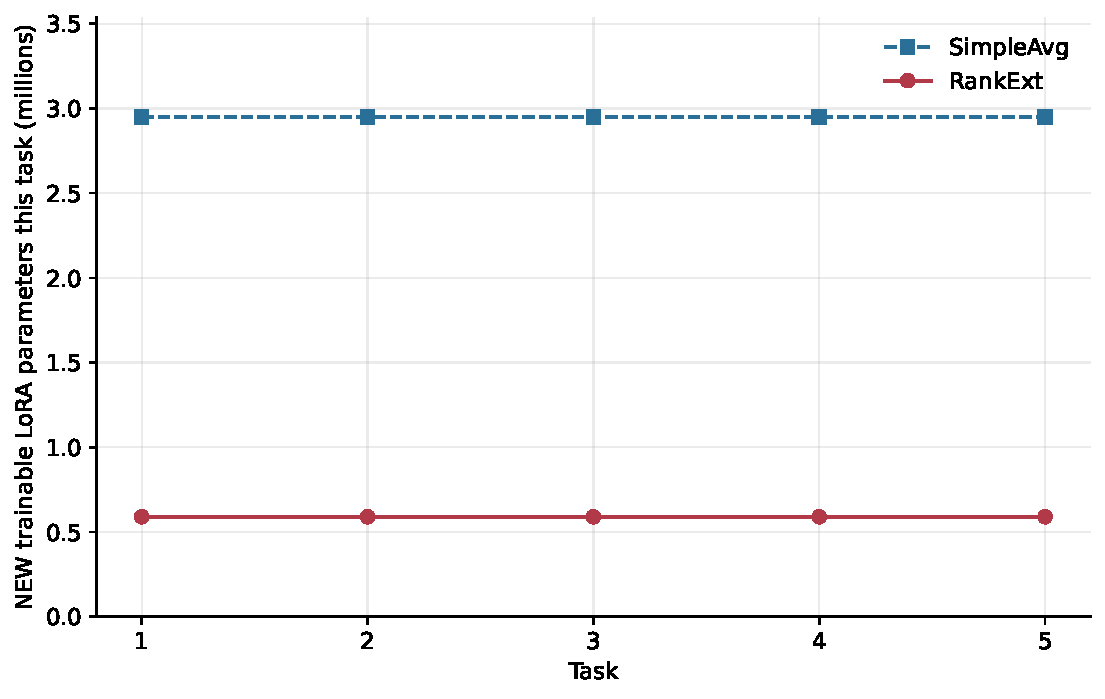
\includegraphics[width=0.8\textwidth]{figures/chapter5/cifar100_trainable_lora_params_per_task.pdf}
\caption[New trainable LoRA parameters per task]{New trainable LoRA
parameters introduced at each task, both families.}
\label{fig:ch5-trainable-params}
\end{figure}

At every task, RankExt trains fewer new parameters than SimpleAvg (589{,}824
vs.\ 2{,}949{,}120, both constant across tasks,
Figure~\ref{fig:ch5-trainable-params}). Summed across the training
sequence, RankExt's cumulative adapter reaches 2{,}949{,}120 parameters by
the final task, exactly matching its own final active rank (80), because
each of its five blocks is trained exactly once and never retrained.
SimpleAvg's five specialists, trained independently, together comprise
14{,}745{,}600 LoRA parameters over the training sequence; this is a
training-time quantity only, since the specialists are not retained
separately at deployment.

The two families also differ in \emph{how} their final adaptation is
deployed, not only in how many parameters it touches during training. In
the evaluated implementation, SimpleAvg is fused into the base weights,
whereas RankExt is retained in its low-rank additive form. SimpleAvg's merge
step averages each of its five specialists' dense
per-module weight updates and adds the averaged update directly into a copy
of the pretrained base model's own weight tensors; no separate low-rank
adapter object survives this step. If this averaged update is fused
directly into the base weights, the deployed model requires no additional
adapter parameters beyond its new 76{,}900-parameter classifier; if the
dense update is instead stored separately from an unmodified base
checkpoint (for example, for reproducibility or versioning), it occupies
14{,}155{,}776 values --- larger than the 2{,}949{,}120-parameter low-rank
form it was derived from, since the averaging step operates on dense, not
low-rank, matrices. RankExt's cumulative adapter, by contrast, is kept in
low-rank, additive form at every step, including the final one: in the
evaluated implementation its 2{,}949{,}120 parameters are not fused into the
base model's weights and remain separable from them. This chapter
reports both quantities and both deployment forms without concluding that
either family is more parameter-efficient in general; the two represent
different trade-offs between training-time parameter volume and
deployed-model structure, examined further in
Chapter~\ref{ch:discussion-conclusion}.

\section{Ablation and Refinement Results}
\label{sec:ch5-ablation}

This section reports a controlled refinement of two hyperparameters, run
separately from the primary benchmark as \textbf{the refinement experiment} and never
merged into Table~\ref{tab:ch5-main-compact} or any of the per-family tables
above. The refinement experiment changes exactly two settings relative to the primary benchmark, each
affecting one family: SimpleAvg's FactorOrth coefficient ($\lambda$) is
lowered from 20 to 1; RankExt's classifier-head learning-rate multiplier is
raised from $\times1$ to $\times2$. Every other setting is unchanged. The
two changes are family-specific and are evaluated separately against their
corresponding primary-benchmark configurations. Both comparisons below are
single-seed, controlled, two-run comparisons --- not a replication of the
primary benchmark itself.

\textbf{SimpleAvg FactorOrth, $\lambda=20$ vs.\ $\lambda=1$.}

\begin{table}[htbp]
\centering
\begin{tabularx}{\textwidth}{@{}>{\raggedright\arraybackslash}X r r r@{}}
\toprule
\textbf{Variant} & \shortstack[r]{\textbf{$\lambda=20$}\\\textbf{(the primary benchmark)}} & \shortstack[r]{\textbf{$\lambda=1$}\\\textbf{(the refinement experiment)}} & \textbf{$\Delta$ (pp)} \\
\midrule
SimpleAvg + FactorOrth & 74.02 & 73.80 & $-$0.22 \\
SimpleAvg + FactorOrth + KD & 73.22 & 74.64 & +1.42 \\
\bottomrule
\end{tabularx}
\caption[SimpleAvg FactorOrth $\lambda$ ablation]{SimpleAvg FactorOrth
(dense-update formulation) coefficient ablation, the primary benchmark ($\lambda=20$) vs.\ the refinement experiment
($\lambda=1$).}
\label{tab:ch5-sa-factororth-ablation}
\end{table}

Lowering $\lambda$ from 20 to 1 does not improve the pure FactorOrth
variant's all-seen accuracy; it is 0.22 percentage points lower at
$\lambda=1$ than at $\lambda=20$, and both values remain below plain
SimpleAvg (75.16\%, Table~\ref{tab:ch5-main-compact}). The FactorOrth+KD
variant is 1.42 points higher at $\lambda=1$ than at $\lambda=20$. Lowering
$\lambda$ therefore produced mixed effects and does not establish a superior
setting; the primary benchmark retains $\lambda=20$. This chapter reports
both deltas as observed, single-seed results; their interpretation is discussed in
Chapter~\ref{ch:discussion-conclusion}.

\textbf{RankExt classifier-head learning rate, $\times1$ vs.\ $\times2$.}

\begin{table}[htbp]
\centering
\begin{tabularx}{\textwidth}{@{}>{\raggedright\arraybackslash}X r r r@{}}
\toprule
\textbf{Variant} & \shortstack[r]{\textbf{$\times1$}\\\textbf{(the primary benchmark)}} & \shortstack[r]{\textbf{$\times2$}\\\textbf{(the refinement experiment)}} & \textbf{$\Delta$ (pp)} \\
\midrule
RankExt & 34.99 & 42.02 & +7.03 \\
RankExt + KD + Protect & 65.01 & 68.50 & +3.49 \\
RankExt + FactorOrth & 41.00 & 43.40 & +2.40 \\
RankExt + FactorOrth + KD + Protect & 70.76 & 67.92 & \textbf{$-$2.84} \\
\bottomrule
\end{tabularx}
\caption[RankExt head-LR ablation]{RankExt classifier-head learning-rate
multiplier ablation, the primary benchmark ($\times1$) vs.\ the refinement experiment ($\times2$).}
\label{tab:ch5-rankext-headlr-ablation}
\end{table}

Raising the RankExt classifier-head learning-rate multiplier from
$\times1$ to $\times2$ improves three of the four RankExt variants relative
to their primary-benchmark counterparts (+2.40 to +7.03 percentage points). The
fourth --- the combined configuration, the strongest RankExt result in the
primary benchmark (Table~\ref{tab:ch5-rankext}) --- decreases, from 70.76\%
to 67.92\%, a change of $-$2.84 percentage points. This is reported here as
an observed, single-seed result, not as evidence that the $\times2$ setting
is worse in general: the combined configuration's other metrics move in
mixed directions at $\times2$ (first-task accuracy rises from 60.70\% to
67.75\%; BWT improves from $-$0.1584 to $-$0.0532; forgetting improves from
0.2474 to 0.1289; later-tasks-mean accuracy falls from 73.28\% to 67.96\%),
a pattern reported factually here and interpreted in
Chapter~\ref{ch:discussion-conclusion}. This chapter does not claim that a
classifier-head learning-rate multiplier of $\times2$ is globally better
than $\times1$ for RankExt; the evidence is mixed across the four
configurations tested.

The $\times2$ setting was chosen after a small, reduced-scale local probe
of the combined RankExt configuration (2 tasks, 2 epochs per task, 10--15
images per class) favoured it; this probe is not benchmark evidence. Its
preference did not fully transfer to the full five-task continual
benchmark, where the strongest combined RankExt configuration regressed
(Chapter~\ref{ch:discussion-conclusion}).

\textbf{Protocol diagnostic: $4\times25$.} A separate, earlier single-seed
run (seed 42, native class order) evaluated the four RankExt configurations
under a $4\times25$ protocol: four steps of 25 classes each, covering the
same 100 classes. It uses the same RankExt implementation, full-output
knowledge distillation ($T=2$, weight 1.0), projected feature protection on
the KD-bearing configurations, factor-space FactorOrth ($\lambda=50$),
classifier-head learning-rate multiplier $\times1$, and classifier
rescaling as the primary benchmark, but differs in two further respects:
7 rather than 9 epochs per step, and a rank-20 rather than rank-16 block per
step (cumulative schedule $[20,40,60,80]$, so the final cumulative rank
remains 80). Table~\ref{tab:ch5-protocol-diag} compares final all-seen
accuracy.

\begin{table}[htbp]
\centering
\begin{tabularx}{\textwidth}{@{}X r r r@{}}
\toprule
\textbf{Method} & \shortstack[r]{\textbf{$5\times20$}\\\textbf{all-seen (\%)}} & \shortstack[r]{\textbf{$4\times25$}\\\textbf{all-seen (\%)}} & \shortstack[r]{\textbf{$\Delta$ ($4\times25-5\times20$)}\\\textbf{(pp)}} \\
\midrule
RankExt & 34.99 & 35.51 & +0.52 \\
RankExt + KD + Protect & 65.01 & 72.73 & +7.72 \\
RankExt + FactorOrth & 41.00 & 42.12 & +1.12 \\
RankExt + FactorOrth + KD + Protect & 70.76 & 73.62 & +2.86 \\
\bottomrule
\end{tabularx}
\caption[RankExt $4\times25$ protocol diagnostic]{RankExt final all-seen
accuracy under the primary $5\times20$ protocol and a secondary $4\times25$
protocol diagnostic (single seed, seed 42). The $4\times25$ run also uses
7 epochs per step and rank-20 increments ($[20,40,60,80]$); it is therefore
not a controlled single-factor comparison.}
\label{tab:ch5-protocol-diag}
\end{table}

This secondary protocol diagnostic changes the incremental partition from
five 20-class steps to four 25-class steps. It is therefore not a direct
replacement for the canonical benchmark, but provides a compact indication
of how RankExt behaves under a shallower continual sequence: all four
configurations reach a higher all-seen accuracy in this run, while plain
RankExt and FactorOrth-only RankExt remain far below the two KD+Protect
configurations.

\section{Summary and Limitations}
\label{sec:ch5-summary}

\begin{table}[htbp]
\centering
\begin{tabularx}{\textwidth}{@{}X r r r r r r@{}}
\toprule
\textbf{Method} & \textbf{All-seen} & \textbf{First-task} & \textbf{Later-tasks} & \textbf{Restricted} & \textbf{BWT} & \textbf{Forgetting} \\
\midrule
SimpleAvg & 75.16 & 77.75 & 74.51 & 92.28 & $-$0.2122 & --- \\
SimpleAvg + KD & 75.21 & 68.25 & 76.95 & 92.86 & $-$0.2001 & --- \\
SimpleAvg + FactorOrth & 74.02 & 76.60 & 73.38 & 91.97 & $-$0.2268 & --- \\
SimpleAvg + FactorOrth + KD & 73.22 & 57.55 & 77.14 & 92.96 & $-$0.2424 & --- \\
RankExt & 34.99 & 11.70 & 40.81 & 91.03 & $-$0.7527 & 0.8130 \\
RankExt + KD + Protect & 65.01 & 62.35 & 65.67 & 94.10 & $-$0.2574 & 0.3269 \\
RankExt + FactorOrth & 41.00 & 9.85 & 48.79 & 93.03 & $-$0.6789 & 0.7646 \\
RankExt + FactorOrth + KD + Protect & 70.76 & 60.70 & 73.28 & 94.78 & $-$0.1584 & 0.2474 \\
\bottomrule
\end{tabularx}
\caption[Extended main benchmark table]{Extended main-benchmark table: all
eight methods, all six metrics. All accuracy columns in percent. BWT and
forgetting are defined in Section~\ref{sec:ch5-protocol}, including the
evaluation stage (before or after classifier rescaling) of each term.}
\label{tab:ch5-main-extended}
\end{table}

\textbf{Ranking, restated concisely.} SimpleAvg's four variants cluster
within a 1.99 percentage-point band (73.22\%--75.21\%), with no auxiliary
configuration producing a clear all-seen improvement over the plain baseline
(Section~\ref{sec:ch5-simpleavg}). RankExt's four variants span a
35.77-point band (34.99\%--70.76\%); the largest observed improvement within
RankExt is associated with the KD+Protect-bearing configurations, and the
combined configuration reaches the highest observed RankExt result in this
run (70.76\%), 4.45 percentage points below the highest observed SimpleAvg
result in this run (75.21\%). RankExt's restricted accuracy remains high
(91.03\%--94.78\%) across all four configurations even where all-seen
accuracy is low, indicating that within-task discrimination is retained
more consistently than task-agnostic discrimination
(Section~\ref{sec:ch5-stability}). Parameter-efficiency accounting
(Section~\ref{sec:ch5-efficiency}) shows the two families reach comparably
sized final adapters through structurally different training and deployment
paths. A controlled refinement of two hyperparameters
(Section~\ref{sec:ch5-ablation}) improves three of the four RankExt
configurations but not the strongest one, and has mixed effects on
SimpleAvg's two FactorOrth variants. On CUB-200-2011
(Section~\ref{sec:ch5-cub}), the same qualitative family-level pattern is
observed: plain SimpleAvg (69.47\%) is not improved by any auxiliary
configuration, while RankExt rises from 20.26\% to 63.43\% with the
combined configuration.

\textbf{Limitations.} Every result presented as primary in this chapter ---
the eight-method benchmark of Section~\ref{sec:ch5-main-results}, the
per-family analyses of Sections~\ref{sec:ch5-simpleavg}--\ref{sec:ch5-efficiency},
and the refinement and protocol-diagnostic comparisons of
Section~\ref{sec:ch5-ablation} --- is a \textbf{single-seed (seed 42)}
result, and so is the CUB-200-2011 evaluation of
Section~\ref{sec:ch5-cub}. The CUB-200-2011 results add a second dataset
but do not replace repeated-seed evidence, and because the CUB-200-2011
configuration also changes the RankExt classifier-head learning rate, they
support qualitative rather than controlled cross-dataset conclusions. The reported benchmark and refinement results are single-seed
observations; no confidence intervals or statistical-significance claims
are made. Differences reported here, including the 4.45-percentage-point
SimpleAvg-vs-RankExt gap and the RankExt combined arm's $-$2.84-point change
under the head-learning-rate refinement, are this run's observed outcome.
Best-epoch selection (by validation cross-entropy, per method and per task)
means that ``final'' accuracy in this chapter is not uniformly the literal
last-epoch checkpoint for every method. The forgetting values are
reproduced exactly from the $R_{i,j}$ matrices of
Section~\ref{sec:ch5-rankext}. The BWT values are not, and the reason is
known: BWT's end-of-sequence term is measured after classifier rescaling,
whereas the final row of $R_{i,j}$ is measured before it
(Section~\ref{sec:ch5-protocol}). Substituting the post-rescaling final
accuracies for the final row of $R_{i,j}$ reproduces the reported BWT values
exactly for all four RankExt configurations; using the pre-rescaling final
row instead yields values between 0.060 and 0.089 lower.

Interpretation of the mechanisms behind these results --- why SimpleAvg's
auxiliary losses do not help, why RankExt's failure is concentrated in
open- rather than restricted-accuracy, why the head-learning-rate refinement
helps three RankExt configurations but not the fourth, and what the
parameter-efficiency and $R_{i,j}$ evidence together suggest about the two
families' underlying architectures --- is developed in
Chapter~\ref{ch:discussion-conclusion}.
